\documentclass[twoside]{book}

% Packages required by doxygen
\usepackage{fixltx2e}
\usepackage{calc}
\usepackage{doxygen}
\usepackage[export]{adjustbox} % also loads graphicx
\usepackage{graphicx}
\usepackage[utf8]{inputenc}
\usepackage{makeidx}
\usepackage{multicol}
\usepackage{multirow}
\PassOptionsToPackage{warn}{textcomp}
\usepackage{textcomp}
\usepackage[nointegrals]{wasysym}
\usepackage[table]{xcolor}

% Font selection
\usepackage[T1]{fontenc}
\usepackage[scaled=.90]{helvet}
\usepackage{courier}
\usepackage{amssymb}
\usepackage{sectsty}
\renewcommand{\familydefault}{\sfdefault}
\allsectionsfont{%
  \fontseries{bc}\selectfont%
  \color{darkgray}%
}
\renewcommand{\DoxyLabelFont}{%
  \fontseries{bc}\selectfont%
  \color{darkgray}%
}
\newcommand{\+}{\discretionary{\mbox{\scriptsize$\hookleftarrow$}}{}{}}

% Page & text layout
\usepackage{geometry}
\geometry{%
  a4paper,%
  top=2.5cm,%
  bottom=2.5cm,%
  left=2.5cm,%
  right=2.5cm%
}
\tolerance=750
\hfuzz=15pt
\hbadness=750
\setlength{\emergencystretch}{15pt}
\setlength{\parindent}{0cm}
\setlength{\parskip}{3ex plus 2ex minus 2ex}
\makeatletter
\renewcommand{\paragraph}{%
  \@startsection{paragraph}{4}{0ex}{-1.0ex}{1.0ex}{%
    \normalfont\normalsize\bfseries\SS@parafont%
  }%
}
\renewcommand{\subparagraph}{%
  \@startsection{subparagraph}{5}{0ex}{-1.0ex}{1.0ex}{%
    \normalfont\normalsize\bfseries\SS@subparafont%
  }%
}
\makeatother

% Headers & footers
\usepackage{fancyhdr}
\pagestyle{fancyplain}
\fancyhead[LE]{\fancyplain{}{\bfseries\thepage}}
\fancyhead[CE]{\fancyplain{}{}}
\fancyhead[RE]{\fancyplain{}{\bfseries\leftmark}}
\fancyhead[LO]{\fancyplain{}{\bfseries\rightmark}}
\fancyhead[CO]{\fancyplain{}{}}
\fancyhead[RO]{\fancyplain{}{\bfseries\thepage}}
\fancyfoot[LE]{\fancyplain{}{}}
\fancyfoot[CE]{\fancyplain{}{}}
\fancyfoot[RE]{\fancyplain{}{\bfseries\scriptsize Generated by Doxygen }}
\fancyfoot[LO]{\fancyplain{}{\bfseries\scriptsize Generated by Doxygen }}
\fancyfoot[CO]{\fancyplain{}{}}
\fancyfoot[RO]{\fancyplain{}{}}
\renewcommand{\footrulewidth}{0.4pt}
\renewcommand{\chaptermark}[1]{%
  \markboth{#1}{}%
}
\renewcommand{\sectionmark}[1]{%
  \markright{\thesection\ #1}%
}

% Indices & bibliography
\usepackage{natbib}
\usepackage[titles]{tocloft}
\setcounter{tocdepth}{3}
\setcounter{secnumdepth}{5}
\makeindex

% Hyperlinks (required, but should be loaded last)
\usepackage{ifpdf}
\ifpdf
  \usepackage[pdftex,pagebackref=true]{hyperref}
\else
  \usepackage[ps2pdf,pagebackref=true]{hyperref}
\fi
\hypersetup{%
  colorlinks=true,%
  linkcolor=blue,%
  citecolor=blue,%
  unicode%
}

% Custom commands
\newcommand{\clearemptydoublepage}{%
  \newpage{\pagestyle{empty}\cleardoublepage}%
}

\usepackage{caption}
\captionsetup{labelsep=space,justification=centering,font={bf},singlelinecheck=off,skip=4pt,position=top}

%===== C O N T E N T S =====

\begin{document}

% Titlepage & ToC
\hypersetup{pageanchor=false,
             bookmarksnumbered=true,
             pdfencoding=unicode
            }
\pagenumbering{alph}
\begin{titlepage}
\vspace*{7cm}
\begin{center}%
{\Large Robot }\\
\vspace*{1cm}
{\large Generated by Doxygen 1.8.13}\\
\end{center}
\end{titlepage}
\clearemptydoublepage
\pagenumbering{roman}
\tableofcontents
\clearemptydoublepage
\pagenumbering{arabic}
\hypersetup{pageanchor=true}

%--- Begin generated contents ---
\chapter{Class Index}
\section{Class List}
Here are the classes, structs, unions and interfaces with brief descriptions\+:\begin{DoxyCompactList}
\item\contentsline{section}{\hyperlink{class_battery}{Battery} }{\pageref{class_battery}}{}
\item\contentsline{section}{\hyperlink{class_bluetooth}{Bluetooth} }{\pageref{class_bluetooth}}{}
\item\contentsline{section}{\hyperlink{class_button}{Button} }{\pageref{class_button}}{}
\item\contentsline{section}{\hyperlink{class_distance}{Distance} }{\pageref{class_distance}}{}
\item\contentsline{section}{\hyperlink{class_filters}{Filters} }{\pageref{class_filters}}{}
\item\contentsline{section}{\hyperlink{class_i_m_u}{I\+MU} }{\pageref{class_i_m_u}}{}
\item\contentsline{section}{\hyperlink{class_line}{Line} }{\pageref{class_line}}{}
\item\contentsline{section}{\hyperlink{class_motor}{Motor} }{\pageref{class_motor}}{}
\item\contentsline{section}{\hyperlink{class_m_p_u9250}{M\+P\+U9250} }{\pageref{class_m_p_u9250}}{}
\item\contentsline{section}{\hyperlink{class_robot}{Robot} }{\pageref{class_robot}}{}
\item\contentsline{section}{\hyperlink{class_r_o_s_interface}{R\+O\+S\+Interface} }{\pageref{class_r_o_s_interface}}{}
\end{DoxyCompactList}

\chapter{Class Documentation}
\hypertarget{class_battery}{}\section{Battery Class Reference}
\label{class_battery}\index{Battery@{Battery}}
\subsection*{Public Member Functions}
\begin{DoxyCompactItemize}
\item 
\mbox{\Hypertarget{class_battery_a36a6234c583e3b3506f4a77e3eb49989}\label{class_battery_a36a6234c583e3b3506f4a77e3eb49989}} 
\hyperlink{class_battery_a36a6234c583e3b3506f4a77e3eb49989}{Battery} ()
\begin{DoxyCompactList}\small\item\em Construct a new \hyperlink{class_battery}{Battery}\+:\+: \hyperlink{class_battery}{Battery} object. \end{DoxyCompactList}\item 
float \hyperlink{class_battery_acb115333af9667ce02138fd00afa93ae}{get\+Voltage} ()
\begin{DoxyCompactList}\small\item\em Returns the current battery voltage. \end{DoxyCompactList}\end{DoxyCompactItemize}


\subsection{Member Function Documentation}
\mbox{\Hypertarget{class_battery_acb115333af9667ce02138fd00afa93ae}\label{class_battery_acb115333af9667ce02138fd00afa93ae}} 
\index{Battery@{Battery}!get\+Voltage@{get\+Voltage}}
\index{get\+Voltage@{get\+Voltage}!Battery@{Battery}}
\subsubsection{\texorpdfstring{get\+Voltage()}{getVoltage()}}
{\footnotesize\ttfamily float Battery\+::get\+Voltage (\begin{DoxyParamCaption}{ }\end{DoxyParamCaption})}



Returns the current battery voltage. 

\begin{DoxyReturn}{Returns}
float \hyperlink{class_battery}{Battery} voltage. 
\end{DoxyReturn}


The documentation for this class was generated from the following files\+:\begin{DoxyCompactItemize}
\item 
Battery.\+h\item 
Battery.\+cpp\end{DoxyCompactItemize}

\hypertarget{class_bluetooth}{}\section{Bluetooth Class Reference}
\label{class_bluetooth}\index{Bluetooth@{Bluetooth}}
\subsection*{Public Member Functions}
\begin{DoxyCompactItemize}
\item 
\mbox{\Hypertarget{class_bluetooth_a13f5e5d1fda538635921f86d79e3499f}\label{class_bluetooth_a13f5e5d1fda538635921f86d79e3499f}} 
void {\bfseries rename} (const char $\ast$name)
\item 
\mbox{\Hypertarget{class_bluetooth_a130166e793fa6ea032fa7615c0aa9ff3}\label{class_bluetooth_a130166e793fa6ea032fa7615c0aa9ff3}} 
void {\bfseries control} ()
\end{DoxyCompactItemize}


The documentation for this class was generated from the following files\+:\begin{DoxyCompactItemize}
\item 
Bluetooth.\+h\item 
Bluetooth.\+cpp\end{DoxyCompactItemize}

\hypertarget{class_button}{}\section{Button Class Reference}
\label{class_button}\index{Button@{Button}}
\subsection*{Public Member Functions}
\begin{DoxyCompactItemize}
\item 
\mbox{\Hypertarget{class_button_a5aa424a69c7923ca5896c465d775bed1}\label{class_button_a5aa424a69c7923ca5896c465d775bed1}} 
uint8\+\_\+t {\bfseries pressed} ()
\item 
\mbox{\Hypertarget{class_button_a01e300b2b63ac4b3014aa5a9819d7366}\label{class_button_a01e300b2b63ac4b3014aa5a9819d7366}} 
void {\bfseries wait} ()
\item 
\mbox{\Hypertarget{class_button_af1464b95c6e43e125904b46670272ed2}\label{class_button_af1464b95c6e43e125904b46670272ed2}} 
void {\bfseries press} ()
\end{DoxyCompactItemize}


The documentation for this class was generated from the following files\+:\begin{DoxyCompactItemize}
\item 
Button.\+h\item 
Button.\+cpp\end{DoxyCompactItemize}

\hypertarget{class_distance}{}\section{Distance Class Reference}
\label{class_distance}\index{Distance@{Distance}}
\subsection*{Public Member Functions}
\begin{DoxyCompactItemize}
\item 
\mbox{\Hypertarget{class_distance_a2690bae35cc62eca885908f3e66bf223}\label{class_distance_a2690bae35cc62eca885908f3e66bf223}} 
void {\bfseries calibrate} (int16\+\_\+t duration)
\item 
\mbox{\Hypertarget{class_distance_a95ceac083560337294bae7f3af74ce11}\label{class_distance_a95ceac083560337294bae7f3af74ce11}} 
float {\bfseries get\+Distance} (uint8\+\_\+t sensor)
\item 
\mbox{\Hypertarget{class_distance_ab551cbc104a827328d82eab4b75df282}\label{class_distance_ab551cbc104a827328d82eab4b75df282}} 
void {\bfseries read\+Calibrated} ()
\item 
\mbox{\Hypertarget{class_distance_aee6d12acb22f7e63088c69ccaafd0ffe}\label{class_distance_aee6d12acb22f7e63088c69ccaafd0ffe}} 
void {\bfseries read\+Calibrated} (uint8\+\_\+t i)
\item 
\mbox{\Hypertarget{class_distance_abae4e3129dbae11894dd5989278a2f46}\label{class_distance_abae4e3129dbae11894dd5989278a2f46}} 
void {\bfseries read\+Raw} ()
\item 
\mbox{\Hypertarget{class_distance_a3fd2a750002215e47abcf426c90f1bab}\label{class_distance_a3fd2a750002215e47abcf426c90f1bab}} 
void {\bfseries read\+Raw} (uint8\+\_\+t i)
\end{DoxyCompactItemize}
\subsection*{Public Attributes}
\begin{DoxyCompactItemize}
\item 
\mbox{\Hypertarget{class_distance_ac7a125bda4d0a1051a65432e6a81df80}\label{class_distance_ac7a125bda4d0a1051a65432e6a81df80}} 
int16\+\_\+t {\bfseries sensors\+Raw} \mbox{[}6\mbox{]} = \{0, 0, 0, 0, 0, 0\}
\item 
\mbox{\Hypertarget{class_distance_a45aa36c346c776c07c4c571afb0b6d07}\label{class_distance_a45aa36c346c776c07c4c571afb0b6d07}} 
int16\+\_\+t {\bfseries sensors\+Min} \mbox{[}6\mbox{]} = \{1023, 1023, 1023, 1023, 1023, 1023\}
\item 
\mbox{\Hypertarget{class_distance_ad297543b8b6594b754fc59c520c535de}\label{class_distance_ad297543b8b6594b754fc59c520c535de}} 
int16\+\_\+t {\bfseries sensors\+Max} \mbox{[}6\mbox{]} = \{0, 0, 0, 0, 0, 0\}
\item 
\mbox{\Hypertarget{class_distance_a596e6343629227348becaae10207ba3b}\label{class_distance_a596e6343629227348becaae10207ba3b}} 
float {\bfseries a} \mbox{[}6\mbox{]} = \{0.\+0, 0.\+0, 0.\+0, 0.\+0, 0.\+0, 0.\+0\}
\item 
\mbox{\Hypertarget{class_distance_aee3b683bd9b0d88242618b17a8900ef5}\label{class_distance_aee3b683bd9b0d88242618b17a8900ef5}} 
float {\bfseries b} \mbox{[}6\mbox{]} = \{0.\+0, 0.\+0, 0.\+0, 0.\+0, 0.\+0, 0.\+0\}
\item 
\mbox{\Hypertarget{class_distance_aa0f265e5fe43c3fdd01cf5403350fe05}\label{class_distance_aa0f265e5fe43c3fdd01cf5403350fe05}} 
float {\bfseries sensors\+Calibrated} \mbox{[}6\mbox{]} = \{0, 0, 0, 0, 0, 0\}
\item 
\mbox{\Hypertarget{class_distance_a9952768af57c60288a0733cc07d80e86}\label{class_distance_a9952768af57c60288a0733cc07d80e86}} 
uint32\+\_\+t {\bfseries last\+Update} = 0
\end{DoxyCompactItemize}


The documentation for this class was generated from the following files\+:\begin{DoxyCompactItemize}
\item 
Distance.\+h\item 
Distance.\+cpp\end{DoxyCompactItemize}

\hypertarget{class_filters}{}\section{Filters Class Reference}
\label{class_filters}\index{Filters@{Filters}}
\subsection*{Public Member Functions}
\begin{DoxyCompactItemize}
\item 
\mbox{\Hypertarget{class_filters_a803ebcd6adb5c3cb765a321b0a8bd7fa}\label{class_filters_a803ebcd6adb5c3cb765a321b0a8bd7fa}} 
void {\bfseries Madgwick\+Quaternion\+Update} (float ax, float ay, float az, float gx, float gy, float gz, float mx, float my, float mz)
\item 
\mbox{\Hypertarget{class_filters_a0eb64d0ce636db7e7ca34e8b5da8d50a}\label{class_filters_a0eb64d0ce636db7e7ca34e8b5da8d50a}} 
void {\bfseries Mahony\+Quaternion\+Update} (float ax, float ay, float az, float gx, float gy, float gz, float mx, float my, float mz)
\end{DoxyCompactItemize}
\subsection*{Public Attributes}
\begin{DoxyCompactItemize}
\item 
\mbox{\Hypertarget{class_filters_aa8b3e816dd712cb6a4d34a8eb431162f}\label{class_filters_aa8b3e816dd712cb6a4d34a8eb431162f}} 
float {\bfseries pitch}
\item 
\mbox{\Hypertarget{class_filters_ab6c0b1114d4b6468dea6b77ebea2d17e}\label{class_filters_ab6c0b1114d4b6468dea6b77ebea2d17e}} 
float {\bfseries yaw}
\item 
\mbox{\Hypertarget{class_filters_a8cbbce68157a4b3f14a85bdc9b9b1c1e}\label{class_filters_a8cbbce68157a4b3f14a85bdc9b9b1c1e}} 
float {\bfseries roll}
\item 
\mbox{\Hypertarget{class_filters_a41fc34c7ed2a7036eb60473cbb6f2852}\label{class_filters_a41fc34c7ed2a7036eb60473cbb6f2852}} 
float {\bfseries q} \mbox{[}4\mbox{]} = \{1.\+0f, 0.\+0f, 0.\+0f, 0.\+0f\}
\end{DoxyCompactItemize}


The documentation for this class was generated from the following files\+:\begin{DoxyCompactItemize}
\item 
Filters.\+h\item 
Filters.\+cpp\end{DoxyCompactItemize}

\hypertarget{class_i_m_u}{}\section{I\+MU Class Reference}
\label{class_i_m_u}\index{I\+MU@{I\+MU}}


Collaboration diagram for I\+MU\+:
\nopagebreak
\begin{figure}[H]
\begin{center}
\leavevmode
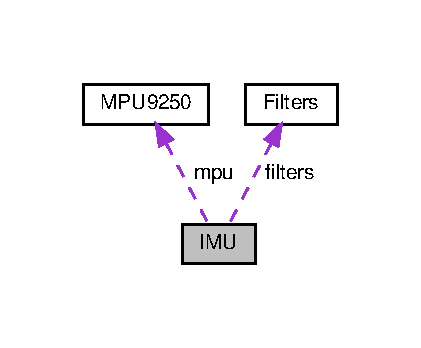
\includegraphics[width=202pt]{class_i_m_u__coll__graph}
\end{center}
\end{figure}
\subsection*{Public Member Functions}
\begin{DoxyCompactItemize}
\item 
\mbox{\Hypertarget{class_i_m_u_ad1d78a07fc6b4a1e36ced1c376512710}\label{class_i_m_u_ad1d78a07fc6b4a1e36ced1c376512710}} 
float {\bfseries get\+Roll} ()
\item 
\mbox{\Hypertarget{class_i_m_u_a62628ef9d9418c9342fc474d575c2aaa}\label{class_i_m_u_a62628ef9d9418c9342fc474d575c2aaa}} 
float {\bfseries get\+Pitch} ()
\item 
\mbox{\Hypertarget{class_i_m_u_a5a66528c1e6b6a80730a9ae880288611}\label{class_i_m_u_a5a66528c1e6b6a80730a9ae880288611}} 
float {\bfseries get\+Yaw} ()
\item 
\mbox{\Hypertarget{class_i_m_u_ab922483ebdc2032cf6801ed45d980a52}\label{class_i_m_u_ab922483ebdc2032cf6801ed45d980a52}} 
float {\bfseries get\+AX} ()
\item 
\mbox{\Hypertarget{class_i_m_u_ad934dd43df8b862c944a7607cf1fd5bc}\label{class_i_m_u_ad934dd43df8b862c944a7607cf1fd5bc}} 
float {\bfseries get\+AY} ()
\item 
\mbox{\Hypertarget{class_i_m_u_a0a0cebfe563d2ccfbdf39122ce703c08}\label{class_i_m_u_a0a0cebfe563d2ccfbdf39122ce703c08}} 
float {\bfseries get\+AZ} ()
\item 
\mbox{\Hypertarget{class_i_m_u_a1e4f460df459755de52fe7143abdf69a}\label{class_i_m_u_a1e4f460df459755de52fe7143abdf69a}} 
float {\bfseries get\+GX} ()
\item 
\mbox{\Hypertarget{class_i_m_u_afb91ddd6436ce75301ce2be523c66d78}\label{class_i_m_u_afb91ddd6436ce75301ce2be523c66d78}} 
float {\bfseries get\+GY} ()
\item 
\mbox{\Hypertarget{class_i_m_u_a8de1988b275a5c273f87569f60f8b228}\label{class_i_m_u_a8de1988b275a5c273f87569f60f8b228}} 
float {\bfseries get\+GZ} ()
\item 
\mbox{\Hypertarget{class_i_m_u_a18860a539a96b26ced52aa26828c4ed7}\label{class_i_m_u_a18860a539a96b26ced52aa26828c4ed7}} 
float {\bfseries get\+MX} ()
\item 
\mbox{\Hypertarget{class_i_m_u_a2bb9d1d0affd6ed32d3c567738317c85}\label{class_i_m_u_a2bb9d1d0affd6ed32d3c567738317c85}} 
float {\bfseries get\+MY} ()
\item 
\mbox{\Hypertarget{class_i_m_u_a867b1a0bae57f6dc9c55bca0cf3f9c17}\label{class_i_m_u_a867b1a0bae57f6dc9c55bca0cf3f9c17}} 
float {\bfseries get\+MZ} ()
\item 
\mbox{\Hypertarget{class_i_m_u_a2be1f7017e9a8747790ffd4a0d116f4c}\label{class_i_m_u_a2be1f7017e9a8747790ffd4a0d116f4c}} 
void {\bfseries calibrate} ()
\end{DoxyCompactItemize}
\subsection*{Public Attributes}
\begin{DoxyCompactItemize}
\item 
\mbox{\Hypertarget{class_i_m_u_ac7b2db5d2aa9f69912509fadec1a6144}\label{class_i_m_u_ac7b2db5d2aa9f69912509fadec1a6144}} 
\hyperlink{class_filters}{Filters} {\bfseries filters} = \hyperlink{class_filters}{Filters}()
\item 
\mbox{\Hypertarget{class_i_m_u_a87ff319ad7422f7c4008c5c3a22c5ac0}\label{class_i_m_u_a87ff319ad7422f7c4008c5c3a22c5ac0}} 
\hyperlink{class_m_p_u9250}{M\+P\+U9250} {\bfseries mpu} = \hyperlink{class_m_p_u9250}{M\+P\+U9250}(Wire, 0x68)
\end{DoxyCompactItemize}


The documentation for this class was generated from the following files\+:\begin{DoxyCompactItemize}
\item 
I\+M\+U.\+h\item 
I\+M\+U.\+cpp\end{DoxyCompactItemize}

\hypertarget{class_line}{}\section{Line Class Reference}
\label{class_line}\index{Line@{Line}}
\subsection*{Public Member Functions}
\begin{DoxyCompactItemize}
\item 
\mbox{\Hypertarget{class_line_a881d9279bdc8f59b5080f73ad00788e3}\label{class_line_a881d9279bdc8f59b5080f73ad00788e3}} 
void {\bfseries calibrate} (int16\+\_\+t duration)
\item 
\mbox{\Hypertarget{class_line_aa0526da82dd7543ac75fc07ee3dbb31c}\label{class_line_aa0526da82dd7543ac75fc07ee3dbb31c}} 
float {\bfseries get\+Position} ()
\item 
\mbox{\Hypertarget{class_line_ace99d3c925c8b71cb967188c029879e7}\label{class_line_ace99d3c925c8b71cb967188c029879e7}} 
float {\bfseries get\+Angle} ()
\item 
\mbox{\Hypertarget{class_line_ad7e330a07e5db282314a9240b3081ba7}\label{class_line_ad7e330a07e5db282314a9240b3081ba7}} 
float {\bfseries set\+Noise\+Threshold} (int16\+\_\+t threshold)
\item 
\mbox{\Hypertarget{class_line_a372f6cc5b268b6baf3629b0042fbfee7}\label{class_line_a372f6cc5b268b6baf3629b0042fbfee7}} 
float {\bfseries set\+Color} (uint8\+\_\+t color)
\item 
\mbox{\Hypertarget{class_line_a972acaef656a4ddfe3bf3e82a2a0f493}\label{class_line_a972acaef656a4ddfe3bf3e82a2a0f493}} 
uint16\+\_\+t {\bfseries get\+Sensor} (uint8\+\_\+t sensor)
\item 
\mbox{\Hypertarget{class_line_a72563901f4a04dc87ceacc7913655bb6}\label{class_line_a72563901f4a04dc87ceacc7913655bb6}} 
float {\bfseries get\+Length} ()
\item 
\mbox{\Hypertarget{class_line_aba3cf991fad6400a3d8735336c509344}\label{class_line_aba3cf991fad6400a3d8735336c509344}} 
void {\bfseries set\+Length} (float length)
\item 
\mbox{\Hypertarget{class_line_a1f1166d184eab9bc6a8445f20d1f26e3}\label{class_line_a1f1166d184eab9bc6a8445f20d1f26e3}} 
void {\bfseries read\+Calibrated} ()
\item 
\mbox{\Hypertarget{class_line_aef792239bcba2dd7db1f71dfd608bd09}\label{class_line_aef792239bcba2dd7db1f71dfd608bd09}} 
void {\bfseries read\+Raw} ()
\end{DoxyCompactItemize}
\subsection*{Public Attributes}
\begin{DoxyCompactItemize}
\item 
\mbox{\Hypertarget{class_line_aceb7cc67fdcf4817b0e69be4e5eb7a58}\label{class_line_aceb7cc67fdcf4817b0e69be4e5eb7a58}} 
int16\+\_\+t {\bfseries sensors\+Raw} \mbox{[}8\mbox{]} = \{0, 0, 0, 0, 0, 0, 0, 0\}
\item 
\mbox{\Hypertarget{class_line_a3b2d5adf497cc8f3edfd7e9f1a87ca7b}\label{class_line_a3b2d5adf497cc8f3edfd7e9f1a87ca7b}} 
int16\+\_\+t {\bfseries sensors\+Min} \mbox{[}8\mbox{]} = \{1023, 1023, 1023, 1023, 1023, 1023, 1023, 1023\}
\item 
\mbox{\Hypertarget{class_line_a4ca4bfe1fcd6875d958601cccc962f67}\label{class_line_a4ca4bfe1fcd6875d958601cccc962f67}} 
int16\+\_\+t {\bfseries sensors\+Max} \mbox{[}8\mbox{]} = \{0, 0, 0, 0, 0, 0, 0, 0\}
\item 
\mbox{\Hypertarget{class_line_a41c4aae2e20fe0bc940e377050f9c1e4}\label{class_line_a41c4aae2e20fe0bc940e377050f9c1e4}} 
int16\+\_\+t {\bfseries sensors\+Calibrated} \mbox{[}8\mbox{]} = \{0, 0, 0, 0, 0, 0, 0, 0\}
\item 
\mbox{\Hypertarget{class_line_a2423d5a551bab0e39848d29b7bb11bb8}\label{class_line_a2423d5a551bab0e39848d29b7bb11bb8}} 
int16\+\_\+t {\bfseries line\+Previous} = 0
\item 
\mbox{\Hypertarget{class_line_a54341251a1179f8bc84563219ae6d990}\label{class_line_a54341251a1179f8bc84563219ae6d990}} 
int16\+\_\+t {\bfseries noise\+Threshold} = 500
\item 
\mbox{\Hypertarget{class_line_a6cc4affae8257c14534495d1b2de19ec}\label{class_line_a6cc4affae8257c14534495d1b2de19ec}} 
uint8\+\_\+t {\bfseries color} = B\+L\+A\+CK
\item 
\mbox{\Hypertarget{class_line_ab7e2334c25ca3ea59df0ef559bd88143}\label{class_line_ab7e2334c25ca3ea59df0ef559bd88143}} 
float {\bfseries length} = 0.\+082
\item 
\mbox{\Hypertarget{class_line_a8059658253032d9bf1a9bb01a4883fc4}\label{class_line_a8059658253032d9bf1a9bb01a4883fc4}} 
uint32\+\_\+t {\bfseries last\+Update} = 0
\end{DoxyCompactItemize}


The documentation for this class was generated from the following files\+:\begin{DoxyCompactItemize}
\item 
Line.\+h\item 
Line.\+cpp\end{DoxyCompactItemize}

\hypertarget{class_motor}{}\section{Motor Class Reference}
\label{class_motor}\index{Motor@{Motor}}
\subsection*{Public Member Functions}
\begin{DoxyCompactItemize}
\item 
\mbox{\Hypertarget{class_motor_a3fabb1dcecaf752268752a0f43fa2fb8}\label{class_motor_a3fabb1dcecaf752268752a0f43fa2fb8}} 
{\bfseries Motor} (uint8\+\_\+t motor)
\item 
\mbox{\Hypertarget{class_motor_a76235bce62e0d77e5346e6e8f7c0cbc5}\label{class_motor_a76235bce62e0d77e5346e6e8f7c0cbc5}} 
float {\bfseries get\+Voltage} ()
\item 
\mbox{\Hypertarget{class_motor_ab4a93f9845eff9d8a480015a623efd79}\label{class_motor_ab4a93f9845eff9d8a480015a623efd79}} 
void {\bfseries set\+Voltage} (float u)
\item 
\mbox{\Hypertarget{class_motor_a16fd26b8314eb4d70fa1910deb482797}\label{class_motor_a16fd26b8314eb4d70fa1910deb482797}} 
float {\bfseries get\+Speed} ()
\item 
\mbox{\Hypertarget{class_motor_a64385407ec4934a908c0257f82b7bea4}\label{class_motor_a64385407ec4934a908c0257f82b7bea4}} 
void {\bfseries set\+Speed} (float w)
\item 
\mbox{\Hypertarget{class_motor_aa74f0ff28a8a9feb8c4c4611cfd401d8}\label{class_motor_aa74f0ff28a8a9feb8c4c4611cfd401d8}} 
void {\bfseries set\+Speed\+Gains} (float kp, float ki, float kd)
\item 
\mbox{\Hypertarget{class_motor_aa1713e2fbb9e21731f37214992837463}\label{class_motor_aa1713e2fbb9e21731f37214992837463}} 
void {\bfseries set\+Speed\+I\+Limit} (float limit)
\item 
\mbox{\Hypertarget{class_motor_ab92163695a7882cdd720117ff68ba6fc}\label{class_motor_ab92163695a7882cdd720117ff68ba6fc}} 
void {\bfseries resetI} ()
\item 
\mbox{\Hypertarget{class_motor_ac53b32c1f6f7585e0ab7ea871af374a5}\label{class_motor_ac53b32c1f6f7585e0ab7ea871af374a5}} 
float {\bfseries get\+Distance} ()
\item 
\mbox{\Hypertarget{class_motor_afff566edc713a0369ca52724168b7a48}\label{class_motor_afff566edc713a0369ca52724168b7a48}} 
void {\bfseries reset\+Distance} ()
\item 
\mbox{\Hypertarget{class_motor_a94587db25ab4933d8e19f51eeeccb7ce}\label{class_motor_a94587db25ab4933d8e19f51eeeccb7ce}} 
float {\bfseries get\+Distance\+Rad} ()
\item 
\mbox{\Hypertarget{class_motor_af98e004e4e7b84ba55afa583427efcea}\label{class_motor_af98e004e4e7b84ba55afa583427efcea}} 
float {\bfseries get\+Diameter} ()
\item 
\mbox{\Hypertarget{class_motor_a40ee451fbda9157a35f7b6ea64f11363}\label{class_motor_a40ee451fbda9157a35f7b6ea64f11363}} 
void {\bfseries set\+Diameter} (float diameter)
\item 
\mbox{\Hypertarget{class_motor_aef53dc289cf7f68db5f07a88cf214f25}\label{class_motor_aef53dc289cf7f68db5f07a88cf214f25}} 
void {\bfseries C\+A\+P\+T\+\_\+\+I\+SR} (uint8\+\_\+t motor)
\item 
\mbox{\Hypertarget{class_motor_a0d6208b43d7c5a88f49c1baf63310606}\label{class_motor_a0d6208b43d7c5a88f49c1baf63310606}} 
void {\bfseries O\+V\+F\+\_\+\+I\+SR} ()
\end{DoxyCompactItemize}


The documentation for this class was generated from the following files\+:\begin{DoxyCompactItemize}
\item 
Motor.\+h\item 
Motor.\+cpp\end{DoxyCompactItemize}

\hypertarget{class_m_p_u9250}{}\section{M\+P\+U9250 Class Reference}
\label{class_m_p_u9250}\index{M\+P\+U9250@{M\+P\+U9250}}
\subsection*{Public Types}
\begin{DoxyCompactItemize}
\item 
\mbox{\Hypertarget{class_m_p_u9250_afef8319c985d9930cd31797263b37585}\label{class_m_p_u9250_afef8319c985d9930cd31797263b37585}} 
enum {\bfseries Gyro\+Range} \{ {\bfseries G\+Y\+R\+O\+\_\+\+R\+A\+N\+G\+E\+\_\+250\+D\+PS}, 
{\bfseries G\+Y\+R\+O\+\_\+\+R\+A\+N\+G\+E\+\_\+500\+D\+PS}, 
{\bfseries G\+Y\+R\+O\+\_\+\+R\+A\+N\+G\+E\+\_\+1000\+D\+PS}, 
{\bfseries G\+Y\+R\+O\+\_\+\+R\+A\+N\+G\+E\+\_\+2000\+D\+PS}
 \}
\item 
\mbox{\Hypertarget{class_m_p_u9250_a1d1d4f36ec5a9cd9cea9e196b02cb0f1}\label{class_m_p_u9250_a1d1d4f36ec5a9cd9cea9e196b02cb0f1}} 
enum {\bfseries Accel\+Range} \{ {\bfseries A\+C\+C\+E\+L\+\_\+\+R\+A\+N\+G\+E\+\_\+2G}, 
{\bfseries A\+C\+C\+E\+L\+\_\+\+R\+A\+N\+G\+E\+\_\+4G}, 
{\bfseries A\+C\+C\+E\+L\+\_\+\+R\+A\+N\+G\+E\+\_\+8G}, 
{\bfseries A\+C\+C\+E\+L\+\_\+\+R\+A\+N\+G\+E\+\_\+16G}
 \}
\item 
\mbox{\Hypertarget{class_m_p_u9250_a7eb38e4553c5cb064169037c6172baa8}\label{class_m_p_u9250_a7eb38e4553c5cb064169037c6172baa8}} 
enum {\bfseries Dlpf\+Bandwidth} \{ \newline
{\bfseries D\+L\+P\+F\+\_\+\+B\+A\+N\+D\+W\+I\+D\+T\+H\+\_\+184\+HZ}, 
{\bfseries D\+L\+P\+F\+\_\+\+B\+A\+N\+D\+W\+I\+D\+T\+H\+\_\+92\+HZ}, 
{\bfseries D\+L\+P\+F\+\_\+\+B\+A\+N\+D\+W\+I\+D\+T\+H\+\_\+41\+HZ}, 
{\bfseries D\+L\+P\+F\+\_\+\+B\+A\+N\+D\+W\+I\+D\+T\+H\+\_\+20\+HZ}, 
\newline
{\bfseries D\+L\+P\+F\+\_\+\+B\+A\+N\+D\+W\+I\+D\+T\+H\+\_\+10\+HZ}, 
{\bfseries D\+L\+P\+F\+\_\+\+B\+A\+N\+D\+W\+I\+D\+T\+H\+\_\+5\+HZ}
 \}
\item 
\mbox{\Hypertarget{class_m_p_u9250_a497013a9b2a7273571fb83c9c2b2266f}\label{class_m_p_u9250_a497013a9b2a7273571fb83c9c2b2266f}} 
enum {\bfseries Lp\+Accel\+Odr} \{ \newline
{\bfseries L\+P\+\_\+\+A\+C\+C\+E\+L\+\_\+\+O\+D\+R\+\_\+0\+\_\+24\+HZ} = 0, 
{\bfseries L\+P\+\_\+\+A\+C\+C\+E\+L\+\_\+\+O\+D\+R\+\_\+0\+\_\+49\+HZ} = 1, 
{\bfseries L\+P\+\_\+\+A\+C\+C\+E\+L\+\_\+\+O\+D\+R\+\_\+0\+\_\+98\+HZ} = 2, 
{\bfseries L\+P\+\_\+\+A\+C\+C\+E\+L\+\_\+\+O\+D\+R\+\_\+1\+\_\+95\+HZ} = 3, 
\newline
{\bfseries L\+P\+\_\+\+A\+C\+C\+E\+L\+\_\+\+O\+D\+R\+\_\+3\+\_\+91\+HZ} = 4, 
{\bfseries L\+P\+\_\+\+A\+C\+C\+E\+L\+\_\+\+O\+D\+R\+\_\+7\+\_\+81\+HZ} = 5, 
{\bfseries L\+P\+\_\+\+A\+C\+C\+E\+L\+\_\+\+O\+D\+R\+\_\+15\+\_\+63\+HZ} = 6, 
{\bfseries L\+P\+\_\+\+A\+C\+C\+E\+L\+\_\+\+O\+D\+R\+\_\+31\+\_\+25\+HZ} = 7, 
\newline
{\bfseries L\+P\+\_\+\+A\+C\+C\+E\+L\+\_\+\+O\+D\+R\+\_\+62\+\_\+50\+HZ} = 8, 
{\bfseries L\+P\+\_\+\+A\+C\+C\+E\+L\+\_\+\+O\+D\+R\+\_\+125\+HZ} = 9, 
{\bfseries L\+P\+\_\+\+A\+C\+C\+E\+L\+\_\+\+O\+D\+R\+\_\+250\+HZ} = 10, 
{\bfseries L\+P\+\_\+\+A\+C\+C\+E\+L\+\_\+\+O\+D\+R\+\_\+500\+HZ} = 11
 \}
\end{DoxyCompactItemize}
\subsection*{Public Member Functions}
\begin{DoxyCompactItemize}
\item 
\mbox{\Hypertarget{class_m_p_u9250_acaf2ae31cfdeb6d47b922996feb55b69}\label{class_m_p_u9250_acaf2ae31cfdeb6d47b922996feb55b69}} 
{\bfseries M\+P\+U9250} (Two\+Wire \&bus, uint8\+\_\+t address)
\item 
\mbox{\Hypertarget{class_m_p_u9250_ab0e26058e7148ebf5af4569138337a02}\label{class_m_p_u9250_ab0e26058e7148ebf5af4569138337a02}} 
int {\bfseries begin} ()
\item 
\mbox{\Hypertarget{class_m_p_u9250_a469a02366142d54fb58e39880ea7fa01}\label{class_m_p_u9250_a469a02366142d54fb58e39880ea7fa01}} 
int {\bfseries set\+Accel\+Range} (Accel\+Range range)
\item 
\mbox{\Hypertarget{class_m_p_u9250_a472679872163e0c4994ae125982d5fd2}\label{class_m_p_u9250_a472679872163e0c4994ae125982d5fd2}} 
int {\bfseries set\+Gyro\+Range} (Gyro\+Range range)
\item 
\mbox{\Hypertarget{class_m_p_u9250_a0b3804d17270a7bfe40f2e31e2e4bdc8}\label{class_m_p_u9250_a0b3804d17270a7bfe40f2e31e2e4bdc8}} 
int {\bfseries set\+Dlpf\+Bandwidth} (Dlpf\+Bandwidth bandwidth)
\item 
\mbox{\Hypertarget{class_m_p_u9250_a969857ba25ba11cc34eb900ca6428817}\label{class_m_p_u9250_a969857ba25ba11cc34eb900ca6428817}} 
int {\bfseries set\+Srd} (uint8\+\_\+t srd)
\item 
\mbox{\Hypertarget{class_m_p_u9250_aff5c0acd0797c79230d78c5e6c8a6321}\label{class_m_p_u9250_aff5c0acd0797c79230d78c5e6c8a6321}} 
int {\bfseries read\+Sensor} ()
\item 
\mbox{\Hypertarget{class_m_p_u9250_ab9daf3fb8328d3fb3ae77a0fa0957a7e}\label{class_m_p_u9250_ab9daf3fb8328d3fb3ae77a0fa0957a7e}} 
float {\bfseries get\+Accel\+X\+\_\+mss} ()
\item 
\mbox{\Hypertarget{class_m_p_u9250_ad3cbdd7b229e429b77c06cfabee778a1}\label{class_m_p_u9250_ad3cbdd7b229e429b77c06cfabee778a1}} 
float {\bfseries get\+Accel\+Y\+\_\+mss} ()
\item 
\mbox{\Hypertarget{class_m_p_u9250_a58a1600a522933cd5cbd9a8f5ffc4536}\label{class_m_p_u9250_a58a1600a522933cd5cbd9a8f5ffc4536}} 
float {\bfseries get\+Accel\+Z\+\_\+mss} ()
\item 
\mbox{\Hypertarget{class_m_p_u9250_a2ec6d66f8a1d381e5a6b558756e3275d}\label{class_m_p_u9250_a2ec6d66f8a1d381e5a6b558756e3275d}} 
float {\bfseries get\+Gyro\+X\+\_\+rads} ()
\item 
\mbox{\Hypertarget{class_m_p_u9250_a187251337b4cfb80683cfaaa65ab9e58}\label{class_m_p_u9250_a187251337b4cfb80683cfaaa65ab9e58}} 
float {\bfseries get\+Gyro\+Y\+\_\+rads} ()
\item 
\mbox{\Hypertarget{class_m_p_u9250_a07f8ccd1907f134d866105e3d5ec5a10}\label{class_m_p_u9250_a07f8ccd1907f134d866105e3d5ec5a10}} 
float {\bfseries get\+Gyro\+Z\+\_\+rads} ()
\item 
\mbox{\Hypertarget{class_m_p_u9250_a65c4f2aace22a783462b0ee9ef5cdd7b}\label{class_m_p_u9250_a65c4f2aace22a783462b0ee9ef5cdd7b}} 
float {\bfseries get\+Mag\+X\+\_\+uT} ()
\item 
\mbox{\Hypertarget{class_m_p_u9250_ac909d3078a23d24d44fb8852f9371c40}\label{class_m_p_u9250_ac909d3078a23d24d44fb8852f9371c40}} 
float {\bfseries get\+Mag\+Y\+\_\+uT} ()
\item 
\mbox{\Hypertarget{class_m_p_u9250_a95b19aa80f3ce812d6ccb87b57475389}\label{class_m_p_u9250_a95b19aa80f3ce812d6ccb87b57475389}} 
float {\bfseries get\+Mag\+Z\+\_\+uT} ()
\item 
\mbox{\Hypertarget{class_m_p_u9250_a3b6cad3768c6153c56fcac4edd3fe792}\label{class_m_p_u9250_a3b6cad3768c6153c56fcac4edd3fe792}} 
float {\bfseries get\+Temperature\+\_\+C} ()
\item 
\mbox{\Hypertarget{class_m_p_u9250_a88596ddf9d0f52ca7b9181706d17217f}\label{class_m_p_u9250_a88596ddf9d0f52ca7b9181706d17217f}} 
int {\bfseries calibrate\+Gyro} ()
\item 
\mbox{\Hypertarget{class_m_p_u9250_a551689391a2bfa5aa4af6f10b586ee76}\label{class_m_p_u9250_a551689391a2bfa5aa4af6f10b586ee76}} 
float {\bfseries get\+Gyro\+Bias\+X\+\_\+rads} ()
\item 
\mbox{\Hypertarget{class_m_p_u9250_a42bd5c0267c0fa180dbc5c332db1ec66}\label{class_m_p_u9250_a42bd5c0267c0fa180dbc5c332db1ec66}} 
float {\bfseries get\+Gyro\+Bias\+Y\+\_\+rads} ()
\item 
\mbox{\Hypertarget{class_m_p_u9250_aa48133a853a679469bfc91235c4a52cf}\label{class_m_p_u9250_aa48133a853a679469bfc91235c4a52cf}} 
float {\bfseries get\+Gyro\+Bias\+Z\+\_\+rads} ()
\item 
\mbox{\Hypertarget{class_m_p_u9250_add18eb9ed44f047f11d75b2f1e44af4b}\label{class_m_p_u9250_add18eb9ed44f047f11d75b2f1e44af4b}} 
void {\bfseries set\+Gyro\+Bias\+X\+\_\+rads} (float bias)
\item 
\mbox{\Hypertarget{class_m_p_u9250_aa4adc28e4c00afdd04d9a0c754ef5cfd}\label{class_m_p_u9250_aa4adc28e4c00afdd04d9a0c754ef5cfd}} 
void {\bfseries set\+Gyro\+Bias\+Y\+\_\+rads} (float bias)
\item 
\mbox{\Hypertarget{class_m_p_u9250_a66bf9a29debfc2de700f77373544c1a7}\label{class_m_p_u9250_a66bf9a29debfc2de700f77373544c1a7}} 
void {\bfseries set\+Gyro\+Bias\+Z\+\_\+rads} (float bias)
\item 
\mbox{\Hypertarget{class_m_p_u9250_ad5f4d08b299f35374d1bca9d7122fcdc}\label{class_m_p_u9250_ad5f4d08b299f35374d1bca9d7122fcdc}} 
int {\bfseries calibrate\+Accel} ()
\item 
\mbox{\Hypertarget{class_m_p_u9250_ab1216d85d53de15fb1f8ddc1e4424318}\label{class_m_p_u9250_ab1216d85d53de15fb1f8ddc1e4424318}} 
float {\bfseries get\+Accel\+Bias\+X\+\_\+mss} ()
\item 
\mbox{\Hypertarget{class_m_p_u9250_a2664ab962bccde644ef528349e1660d6}\label{class_m_p_u9250_a2664ab962bccde644ef528349e1660d6}} 
float {\bfseries get\+Accel\+Scale\+FactorX} ()
\item 
\mbox{\Hypertarget{class_m_p_u9250_af02b9af589591792b6fe7328582e32ef}\label{class_m_p_u9250_af02b9af589591792b6fe7328582e32ef}} 
float {\bfseries get\+Accel\+Bias\+Y\+\_\+mss} ()
\item 
\mbox{\Hypertarget{class_m_p_u9250_ad9b6213723700af8daba00f31840fe16}\label{class_m_p_u9250_ad9b6213723700af8daba00f31840fe16}} 
float {\bfseries get\+Accel\+Scale\+FactorY} ()
\item 
\mbox{\Hypertarget{class_m_p_u9250_ab3421dae6ebe1190407be7a832b6313c}\label{class_m_p_u9250_ab3421dae6ebe1190407be7a832b6313c}} 
float {\bfseries get\+Accel\+Bias\+Z\+\_\+mss} ()
\item 
\mbox{\Hypertarget{class_m_p_u9250_a046579c4492296dce3d3a0cf2e409e96}\label{class_m_p_u9250_a046579c4492296dce3d3a0cf2e409e96}} 
float {\bfseries get\+Accel\+Scale\+FactorZ} ()
\item 
\mbox{\Hypertarget{class_m_p_u9250_acfc8adb5dcfe24eb35f2a82377c0d8a0}\label{class_m_p_u9250_acfc8adb5dcfe24eb35f2a82377c0d8a0}} 
void {\bfseries set\+Accel\+CalX} (float bias, float scale\+Factor)
\item 
\mbox{\Hypertarget{class_m_p_u9250_aa56ca1f8a383ba760188f204a9ef6548}\label{class_m_p_u9250_aa56ca1f8a383ba760188f204a9ef6548}} 
void {\bfseries set\+Accel\+CalY} (float bias, float scale\+Factor)
\item 
\mbox{\Hypertarget{class_m_p_u9250_a9ab03b06b0d01aa4f8588cd9fd6588c6}\label{class_m_p_u9250_a9ab03b06b0d01aa4f8588cd9fd6588c6}} 
void {\bfseries set\+Accel\+CalZ} (float bias, float scale\+Factor)
\item 
\mbox{\Hypertarget{class_m_p_u9250_aba735458296fb277a05efcb1a3ceb761}\label{class_m_p_u9250_aba735458296fb277a05efcb1a3ceb761}} 
int {\bfseries calibrate\+Mag} ()
\item 
\mbox{\Hypertarget{class_m_p_u9250_a9bb3dfd24f86ce01d45cc34759eff5f5}\label{class_m_p_u9250_a9bb3dfd24f86ce01d45cc34759eff5f5}} 
float {\bfseries get\+Mag\+Bias\+X\+\_\+uT} ()
\item 
\mbox{\Hypertarget{class_m_p_u9250_a9ae0353e7326ba32a11422b3bc7b5cee}\label{class_m_p_u9250_a9ae0353e7326ba32a11422b3bc7b5cee}} 
float {\bfseries get\+Mag\+Scale\+FactorX} ()
\item 
\mbox{\Hypertarget{class_m_p_u9250_a7f9328b066c9c07887c5c79fff33554c}\label{class_m_p_u9250_a7f9328b066c9c07887c5c79fff33554c}} 
float {\bfseries get\+Mag\+Bias\+Y\+\_\+uT} ()
\item 
\mbox{\Hypertarget{class_m_p_u9250_a5457ecd92f0c920312af61df0c1bb1b3}\label{class_m_p_u9250_a5457ecd92f0c920312af61df0c1bb1b3}} 
float {\bfseries get\+Mag\+Scale\+FactorY} ()
\item 
\mbox{\Hypertarget{class_m_p_u9250_a23d0c81842120b27af379961b773465f}\label{class_m_p_u9250_a23d0c81842120b27af379961b773465f}} 
float {\bfseries get\+Mag\+Bias\+Z\+\_\+uT} ()
\item 
\mbox{\Hypertarget{class_m_p_u9250_a859590996f4e1673d0f21eabe5e1a2f4}\label{class_m_p_u9250_a859590996f4e1673d0f21eabe5e1a2f4}} 
float {\bfseries get\+Mag\+Scale\+FactorZ} ()
\item 
\mbox{\Hypertarget{class_m_p_u9250_a063be654730f719544be8a7ce39a433c}\label{class_m_p_u9250_a063be654730f719544be8a7ce39a433c}} 
void {\bfseries set\+Mag\+CalX} (float bias, float scale\+Factor)
\item 
\mbox{\Hypertarget{class_m_p_u9250_af85a3badd3f79969c4715fceec962e39}\label{class_m_p_u9250_af85a3badd3f79969c4715fceec962e39}} 
void {\bfseries set\+Mag\+CalY} (float bias, float scale\+Factor)
\item 
\mbox{\Hypertarget{class_m_p_u9250_a36fab1c8d06aa5dcd0e6a4014d7ca5e7}\label{class_m_p_u9250_a36fab1c8d06aa5dcd0e6a4014d7ca5e7}} 
void {\bfseries set\+Mag\+CalZ} (float bias, float scale\+Factor)
\end{DoxyCompactItemize}
\subsection*{Public Attributes}
\begin{DoxyCompactItemize}
\item 
\mbox{\Hypertarget{class_m_p_u9250_a7f80ffcecb0dd28d2353b46f429d2a5f}\label{class_m_p_u9250_a7f80ffcecb0dd28d2353b46f429d2a5f}} 
float {\bfseries \+\_\+ax}
\item 
\mbox{\Hypertarget{class_m_p_u9250_a32369a95df72383edd03fff2c7439233}\label{class_m_p_u9250_a32369a95df72383edd03fff2c7439233}} 
float {\bfseries \+\_\+ay}
\item 
\mbox{\Hypertarget{class_m_p_u9250_aac7e2beff39549eaa82c7d677b8cc42e}\label{class_m_p_u9250_aac7e2beff39549eaa82c7d677b8cc42e}} 
float {\bfseries \+\_\+az}
\item 
\mbox{\Hypertarget{class_m_p_u9250_a9af2d19af34ffdeb2d09f61f43ab62a8}\label{class_m_p_u9250_a9af2d19af34ffdeb2d09f61f43ab62a8}} 
float {\bfseries \+\_\+gx}
\item 
\mbox{\Hypertarget{class_m_p_u9250_a3e4d7f5b0f10fecaf6e4cad3235d6e29}\label{class_m_p_u9250_a3e4d7f5b0f10fecaf6e4cad3235d6e29}} 
float {\bfseries \+\_\+gy}
\item 
\mbox{\Hypertarget{class_m_p_u9250_af68ffa42e0bf808af73b11a9694d4f86}\label{class_m_p_u9250_af68ffa42e0bf808af73b11a9694d4f86}} 
float {\bfseries \+\_\+gz}
\item 
\mbox{\Hypertarget{class_m_p_u9250_a0f8f1f024f8d3b0461385b53022472ac}\label{class_m_p_u9250_a0f8f1f024f8d3b0461385b53022472ac}} 
float {\bfseries \+\_\+hx}
\item 
\mbox{\Hypertarget{class_m_p_u9250_a25695de739e4ca8432995c81592a5ed1}\label{class_m_p_u9250_a25695de739e4ca8432995c81592a5ed1}} 
float {\bfseries \+\_\+hy}
\item 
\mbox{\Hypertarget{class_m_p_u9250_a28763d4c62447190bdb038623c2fc8c6}\label{class_m_p_u9250_a28763d4c62447190bdb038623c2fc8c6}} 
float {\bfseries \+\_\+hz}
\item 
\mbox{\Hypertarget{class_m_p_u9250_a614da2a23f959ed1c3e68bae5389983d}\label{class_m_p_u9250_a614da2a23f959ed1c3e68bae5389983d}} 
float {\bfseries \+\_\+t}
\end{DoxyCompactItemize}


The documentation for this class was generated from the following files\+:\begin{DoxyCompactItemize}
\item 
M\+P\+U9250.\+h\item 
M\+P\+U9250.\+cpp\end{DoxyCompactItemize}

\hypertarget{class_robot}{}\section{Robot Class Reference}
\label{class_robot}\index{Robot@{Robot}}


Collaboration diagram for Robot\+:
\nopagebreak
\begin{figure}[H]
\begin{center}
\leavevmode
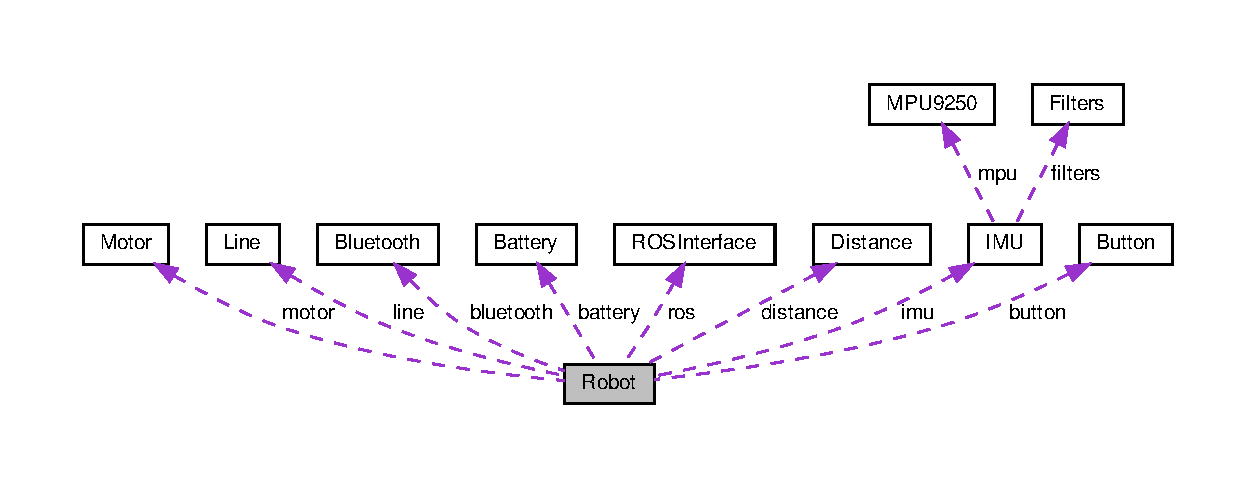
\includegraphics[width=350pt]{class_robot__coll__graph}
\end{center}
\end{figure}
\subsection*{Public Member Functions}
\begin{DoxyCompactItemize}
\item 
\mbox{\Hypertarget{class_robot_a14dfe126ae973d3b9f81fee81a06ac22}\label{class_robot_a14dfe126ae973d3b9f81fee81a06ac22}} 
void {\bfseries stop} ()
\item 
\mbox{\Hypertarget{class_robot_a554d03cb14b5f9eb2baa2175c8ad5f8f}\label{class_robot_a554d03cb14b5f9eb2baa2175c8ad5f8f}} 
void {\bfseries go} (float distance)
\item 
\mbox{\Hypertarget{class_robot_a8ad50ea5e4b3811c8b02201e5a33a580}\label{class_robot_a8ad50ea5e4b3811c8b02201e5a33a580}} 
void {\bfseries go} (float distance, float v)
\item 
\mbox{\Hypertarget{class_robot_a58ed326079adb3283b4129a92fa60097}\label{class_robot_a58ed326079adb3283b4129a92fa60097}} 
void {\bfseries turn} (float angle)
\item 
\mbox{\Hypertarget{class_robot_adda1098497a37d2676dcc64e0021232c}\label{class_robot_adda1098497a37d2676dcc64e0021232c}} 
void {\bfseries turn} (float angle, float w)
\item 
\mbox{\Hypertarget{class_robot_aa5029f34e3f16790254c9a4c46881199}\label{class_robot_aa5029f34e3f16790254c9a4c46881199}} 
void {\bfseries drive} (float v, float w)
\item 
\mbox{\Hypertarget{class_robot_a519f7c469542d18cbc374ab5e60e1a02}\label{class_robot_a519f7c469542d18cbc374ab5e60e1a02}} 
void {\bfseries beep} (int16\+\_\+t frequency, int16\+\_\+t duration)
\item 
\mbox{\Hypertarget{class_robot_a25e965fa83c65b5f1d9bfca6aa5290c4}\label{class_robot_a25e965fa83c65b5f1d9bfca6aa5290c4}} 
void {\bfseries set\+Width} (float width)
\item 
\mbox{\Hypertarget{class_robot_ac3dc9aec2bd1f59314f97a5fbe8db988}\label{class_robot_ac3dc9aec2bd1f59314f97a5fbe8db988}} 
float {\bfseries get\+Speed} ()
\item 
\mbox{\Hypertarget{class_robot_a919a05ad3d64b1d83febe2baccf57c42}\label{class_robot_a919a05ad3d64b1d83febe2baccf57c42}} 
float {\bfseries get\+Angular\+Velocity} ()
\end{DoxyCompactItemize}
\subsection*{Public Attributes}
\begin{DoxyCompactItemize}
\item 
\mbox{\Hypertarget{class_robot_a0a3781e332a541552c93d712f9b3c617}\label{class_robot_a0a3781e332a541552c93d712f9b3c617}} 
\hyperlink{class_button}{Button} {\bfseries button} = \hyperlink{class_button}{Button}()
\item 
\mbox{\Hypertarget{class_robot_a44073d258597157379e95c8b98abca1e}\label{class_robot_a44073d258597157379e95c8b98abca1e}} 
\hyperlink{class_battery}{Battery} {\bfseries battery} = \hyperlink{class_battery}{Battery}()
\item 
\mbox{\Hypertarget{class_robot_a7179be791f542a63d48fb2e97bf8eebb}\label{class_robot_a7179be791f542a63d48fb2e97bf8eebb}} 
\hyperlink{class_motor}{Motor} {\bfseries motor} \mbox{[}2\mbox{]} = \{\hyperlink{class_motor}{Motor}(L\+E\+FT), \hyperlink{class_motor}{Motor}(R\+I\+G\+HT)\}
\item 
\mbox{\Hypertarget{class_robot_a693a004e58b023861750205acf5d1f87}\label{class_robot_a693a004e58b023861750205acf5d1f87}} 
\hyperlink{class_line}{Line} {\bfseries line} = \hyperlink{class_line}{Line}()
\item 
\mbox{\Hypertarget{class_robot_ae272272bc61f3191facdde0d8fa917b0}\label{class_robot_ae272272bc61f3191facdde0d8fa917b0}} 
\hyperlink{class_distance}{Distance} {\bfseries distance} = \hyperlink{class_distance}{Distance}()
\item 
\mbox{\Hypertarget{class_robot_aaccc886d8f992b77c77bad0bf0b87cc4}\label{class_robot_aaccc886d8f992b77c77bad0bf0b87cc4}} 
\hyperlink{class_i_m_u}{I\+MU} {\bfseries imu} = \hyperlink{class_i_m_u}{I\+MU}()
\item 
\mbox{\Hypertarget{class_robot_ad475912c97d313312ed3b3f5a27cdbbb}\label{class_robot_ad475912c97d313312ed3b3f5a27cdbbb}} 
\hyperlink{class_bluetooth}{Bluetooth} {\bfseries bluetooth} = \hyperlink{class_bluetooth}{Bluetooth}()
\item 
\mbox{\Hypertarget{class_robot_a6b65e02af58293548ad020cc121b5dab}\label{class_robot_a6b65e02af58293548ad020cc121b5dab}} 
\hyperlink{class_r_o_s_interface}{R\+O\+S\+Interface} {\bfseries ros} = \hyperlink{class_r_o_s_interface}{R\+O\+S\+Interface}()
\end{DoxyCompactItemize}


The documentation for this class was generated from the following files\+:\begin{DoxyCompactItemize}
\item 
Robot.\+h\item 
Robot.\+cpp\end{DoxyCompactItemize}

\hypertarget{class_r_o_s_interface}{}\section{R\+O\+S\+Interface Class Reference}
\label{class_r_o_s_interface}\index{R\+O\+S\+Interface@{R\+O\+S\+Interface}}
\subsection*{Public Member Functions}
\begin{DoxyCompactItemize}
\item 
\mbox{\Hypertarget{class_r_o_s_interface_ab5d69e3646f227e9eea9c9ffbef3fe32}\label{class_r_o_s_interface_ab5d69e3646f227e9eea9c9ffbef3fe32}} 
void {\bfseries subscribe} ()
\item 
\mbox{\Hypertarget{class_r_o_s_interface_a11b527195b243aa63f58a32175c66f6f}\label{class_r_o_s_interface_a11b527195b243aa63f58a32175c66f6f}} 
void {\bfseries publish\+Battery\+State} ()
\item 
\mbox{\Hypertarget{class_r_o_s_interface_a5c5ee7970a956d6f8839748fc58ba189}\label{class_r_o_s_interface_a5c5ee7970a956d6f8839748fc58ba189}} 
void {\bfseries publish\+Odometry} ()
\item 
\mbox{\Hypertarget{class_r_o_s_interface_a834f215c8126fafc84841b30398e720f}\label{class_r_o_s_interface_a834f215c8126fafc84841b30398e720f}} 
void {\bfseries publish\+Joint\+State} ()
\item 
\mbox{\Hypertarget{class_r_o_s_interface_ad94df75d8e58bf758f60e7eb2f68058a}\label{class_r_o_s_interface_ad94df75d8e58bf758f60e7eb2f68058a}} 
void {\bfseries publish\+I\+MU} ()
\item 
\mbox{\Hypertarget{class_r_o_s_interface_af2ffdcd7a014a2780fab39a8ab62dc29}\label{class_r_o_s_interface_af2ffdcd7a014a2780fab39a8ab62dc29}} 
void {\bfseries publish\+Magnetic\+Field} ()
\end{DoxyCompactItemize}


The documentation for this class was generated from the following files\+:\begin{DoxyCompactItemize}
\item 
R\+O\+S\+Interface.\+h\item 
R\+O\+S\+Interface.\+cpp\end{DoxyCompactItemize}

%--- End generated contents ---

% Index
\backmatter
\newpage
\phantomsection
\clearemptydoublepage
\addcontentsline{toc}{chapter}{Index}
\printindex

\end{document}
